%% LyX 2.3.4 created this file.  For more info, see http://www.lyx.org/.
%% Do not edit unless you really know what you are doing.
\documentclass[a4paper,american]{article}
\usepackage{fancyhdr}
\usepackage{mathptmx}
\renewcommand{\familydefault}{\rmdefault}
\usepackage[T1]{fontenc}
\usepackage[utf8]{inputenc}
\usepackage{graphicx}

\makeatletter

%%%%%%%%%%%%%%%%%%%%%%%%%%%%%% LyX specific LaTeX commands.
\pdfpageheight\paperheight
\pdfpagewidth\paperwidth

\providecommand{\LyX}{L\kern-.1667em\lower.25em\hbox{Y}\kern-.125emX\@}

%%%%%%%%%%%%%%%%%%%%%%%%%%%%%% User specified LaTeX commands.
% used packages
\usepackage[margin=1in]{geometry}
\usepackage[utf8]{inputenc}
\usepackage{lipsum}
\usepackage{afterpage}
\usepackage{xcolor}
\usepackage{pdfpages}
\usepackage{graphicx}
\usepackage{caption}
\usepackage[outputdir=./tmp,newfloat]{minted} % need call 
%<pdflatex -shell-escape>

\usepackage{listings}
%New colors defined below
\definecolor{codegreen}{rgb}{0,0.6,0}
\definecolor{codegray}{rgb}{0.5,0.5,0.5}
\definecolor{codepurple}{rgb}{0.58,0,0.82}
\definecolor{backcolour}{rgb}{0.95,0.95,0.92}
%Code listing style named "mystyle"
\lstdefinestyle{mystyle}{
	backgroundcolor=\color{backcolour},
    commentstyle=\color{codegreen},
	keywordstyle=\color{magenta},
	numberstyle=\tiny\color{codegray},
	stringstyle=\color{codepurple},
	basicstyle=\ttfamily\footnotesize,
	breakatwhitespace=false,         
	breaklines=true,                 
	captionpos=b,                    
	keepspaces=true,                 
	numbers=left,                    
	numbersep=5pt,                  
	showspaces=false,                
	showstringspaces=false,
	showtabs=false,                  
	tabsize=2
}
%"mystyle" code listing set
\lstset{style=mystyle}


\pagestyle{fancy}
\fancyhf{} 	% it clears the header and footer of default "plain" page style
\lhead{\leftmark}
\rhead{\thepage}

\usepackage{hyperref}
\hypersetup{
	colorlinks=true,
	linkcolor=orange,
	urlcolor=magenta
}

\makeatother

\usepackage{babel}
\begin{document}
% cover page
\thispagestyle{empty}
\begin{figure}
	\centering
	\includegraphics[width=1.0\linewidth]{img/lion.png}
	\caption*{how U doin'?}
	\label{cover:lion}
\end{figure}
\pagecolor{pink}
\afterpage{\nopagecolor}
\clearpage
\newpage
\title{{\LaTeX} \& \LyX{} Test}
\author{Mark Taylor}
\date{May 2020}

\maketitle
\tableofcontents 

\section{Insert picture}

Before inserting pictures, add some shit.

\lipsum

\begin{figure}
\includegraphics[width=0.8\paperwidth]{\string"img/The Beatles\string".jpg}'\caption{The Beatles\label{fig:The-Beatles}}
\end{figure}


\section{Insert svg}

\begin{figure}

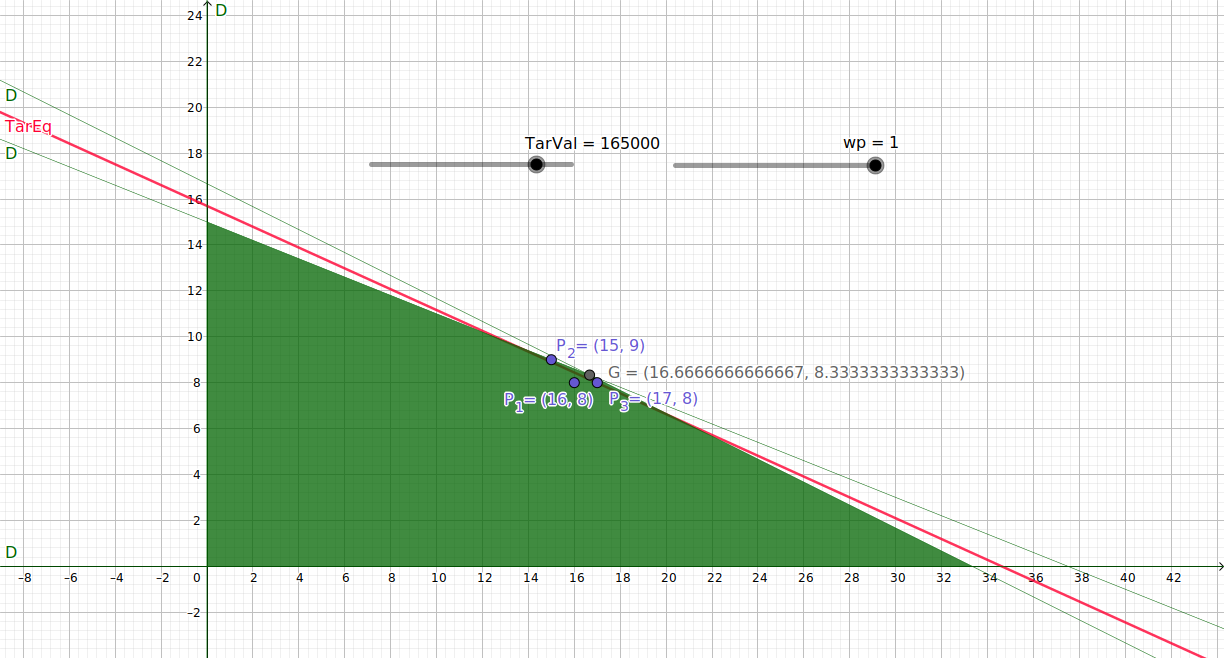
\includegraphics[scale=0.35]{svg/exer11}\caption{\emph{\label{fig:MATLAB-graph-1}MATLAB
 graph 1}}

\end{figure}


\section{Links}

Here is a link to \hyperref[fig:MATLAB-graph-3]{fig 3}. And here is another link that links to \href{https://github.com/How-u-doing}{My GitHub}. 
\noindent See, there's a footnote.\footnote{Hola, this is my GitHub \url{https://github.com/How-u-doing}} Besides, there's graph, click \hyperref[fig:MATLAB-graph-2]{here} to view.

The first and most common use of templates is to supportgeneric programming,
that is, pro-gramming focused on the design, implementation, and use
of general algorithms. Here, ‘‘general’’means that an algorithm can
be designed to accept a wide variety of types as long as they meet
the algorithm’s requirements on its arguments. The template is C++’s
main support for generic pro-gramming. Templates provide (compile-time)
parametric polymorphism.There are many definitions of ‘‘generic programming.’’
Thus, the term can be confusing. How-ev er, in the context of C++,
‘‘generic programming’’ implies an emphasis on the design of generalalgorithms
implemented using templates.Focusing more on generative techniques
(seeing templates as type and function generators) andrelying on type
functions to express compile-time computation are calledtemplate metaprogram-ming,
which is the subject of Chapter 28.The first and most common use of
templates is to supportgeneric programming, that is, pro-gramming
focused on the design, implementation, and use of general algorithms.
Here, ‘‘general’’means that an algorithm can be designed to accept
a wide variety of types as long as they meet thealgorithm’s requirements
on its arguments. The template is C++’s main support for generic pro-gramming.
Templates provide (compile-time) parametric polymorphism.There are
many definitions of ‘‘generic programming.’’ Thus, the term can be
confusing. How-ev er, in the context of C++, ‘‘generic programming’’
implies an emphasis on the design of generalalgorithms implemented
using templates.Focusing more on generative techniques (seeing templates
as type and function generators) andrelying on type functions to express
compile-time computation are calledtemplate metaprogram-ming, which
is the subject of Chapter 28.The first and most common use of templates
is to supportgeneric programming, that is, pro-gramming focused on
the design, implementation, and use of general algorithms. Here, ‘‘general’’means
that an algorithm can be designed to accept a wide variety of types
as long as they meet thealgorithm’s requirements on its arguments.
The template is C++’s main support for generic pro-gramming. Templates
provide (compile-time) parametric polymorphism.There are many definitions
of ‘‘generic programming.’’ Thus, the term can be confusing. How-ev
er, in the context of C++, ‘‘generic programming’’ implies an emphasis
on the design of generalalgorithms implemented using templates.Focusing
more on generative techniques (seeing templates as type and function
generators) andrelying on type functions to express compile-time computation
are calledtemplate metaprogram-ming, which is the subject of Chapter
28.\lipsum

\newpage

\section{Insert graph \& code}

\subsection{Function templates}

ensurehelveticaisembedded\_()Chapter 1Function TemplatesThis chapter
introduces function templates. Function templates are functions that
are parameterizedso that they represent a family of functions.1.1
A First Look at Function TemplatesFunction templates provide a functional
behavior that can be called for different types. In otherwords, a
function template represents a family of functions. The representation
looks a lot like anordinary function, except that some elements of
the function are left undetermined: These elementsare parameterized.
To illustrate, let’s look at a simple example.nsurehelveticaisembedded\_()Chapter
1Function TemplatesThis chapter introduces function templates. Function
templates are functions that are parameterized so that they represent
a family of functions.1.1 A First Look at Function TemplatesFunction
templates provide a functional behavior that can be called for different
types. In other words, a function template represents a family of
functions. The representation looks a lot like anordinary function,
except that some elements of the function are left undetermined: These
elementsare parameterized. To illustrate, let’s look at a simple example.nsurehelveticaisembedded\_()Chapter
1Function TemplatesThis chapter introduces function templates. Function
templates are functions that are parameterizedso that they represent
a family of functions.1.1 A First Look at Function TemplatesFunction
templates provide a functional behavior that can be called for different
types. In otherwords, a function template represents a family of functions.
The representation looks a lot like anordinary function, except that
some elements of the function are left undetermined: These elementsare
parameterized. To illustrate, let’s look at a simple example.nsurehelveticaisembedded\_()Chapter
1Function TemplatesThis chapter introduces function templates. Function
templates are functions that are parameterizedso that they represent
a family of functions.1.1 A First Look at Function TemplatesFunction
templates provide a functional behavior that can be called for different
types. In otherwords, a function template represents a family of functions.
The representation looks a lot like anordinary function, except that
some elements of the function are left undetermined: These elementsare
parameterized. To illustrate, let’s look at a simple example.nsurehelveticaisembedded\_()Chapter
1Function TemplatesThis chapter introduces function templates. Function
templates are functions that are parameterizedso that they represent
a family of functions.1.1 A First Look at Function TemplatesFunction
templates provide a functional behavior that can be called for different
types. In otherwords, a function template represents a family of functions.
The representation looks a lot like anordinary function, except that
some elements of the function are left undetermined: These elementsare
parameterized. To illustrate, let’s look at a simple example.nsurehelveticaisembedded\_()Chapter
1Function TemplatesThis chapter introduces function templates. Function
templates are functions that are parameterizedso that they represent
a family of functions.1.1 A First Look at Function TemplatesFunction
templates provide a functional behavior that can be called for different
types. In otherwords, a function template represents a family of functions.
The representation looks a lot like anordinary function, except that
some elements of the function are left undetermined: These elementsare
parameterized. To illustrate, let’s look at a simple example.Let's
look at \hyperref[fig:The-Beatles]{The Beatles}, or u can click here
to see Figure \ref{fig:The-Beatles}.

Go back to \hyperref[fig:MATLAB-graph-1]{Graph 1} or \hyperref[cover:lion]{cover page}

\begin{figure}
\includegraphics[scale=0.45]{svg/exer8_respective}\caption{\emph{\label{fig:MATLAB-graph-2}MATLAB
 graph 2}}
\end{figure}

\begin{figure}
\includegraphics[scale=0.45]{svg/exer8_combine}\caption{\emph{\label{fig:MATLAB-graph-3}MATLAB
 graph 3}}

\end{figure}


\subsection{Class template}

When we call a function template such asmax()for some arguments, the
template parameters aredetermined by the arguments we pass. If we
pass twoints to the parameter typesT, the C++ compilerhas to conclude
thatTmust beint.However,Tmight only be “part” of the type. For example,
if we declaremax()to use constantreferences:template<typenameT>T max
(Tconst\& a, Tconst\& b)\{returnb < a ? a : b;\}and passint, againTis
deduced asint, because the function parameters match for int const\&.

\subsection{Code}

Following Python code snippet is inserted directly via \LaTeX code
in \LyX . However, we can also import them by source files, see 4.3.1
- 4.3.3. Wanna see \emph{minted \emph{\hyperref[minted_wc]{wc}}}
program?

%Python code highlighting
	\begin{lstlisting}[language=Python, caption=Python example]
	import numpy as np
	
	def incmatrix(genl1,genl2):
		m = len(genl1)
		n = len(genl2)
		M = None #to become the incidence matrix
		VT = np.zeros((n*m,1), int)  #dummy variable
	
	#compute the bitwise xor matrix
	M1 = bitxormatrix(genl1)
	M2 = np.triu(bitxormatrix(genl2),1) 
	
	for i in range(m-1):
		for j in range(i+1, m):
			[r,c] = np.where(M2 == M1[i,j])
	for k in range(len(r)):
		VT[(i)*n + r[k]] = 1;
		VT[(i)*n + c[k]] = 1;
		VT[(j)*n + r[k]] = 1;
		VT[(j)*n + c[k]] = 1;
	
	if M is None:
		M = np.copy(VT)
	else:
		M = np.concatenate((M, VT), 1)
	
	VT = np.zeros((n*m,1), int)
	
	return M
	\end{lstlisting}

\subsubsection{MATLAB Code}

%Importing code from local source file
	\lstinputlisting[language=Octave, 
	caption=Modeling hw4 MATLAB code
	]{src/exer8.m}

\subsubsection{C Code}

1. by \emph{lstlisting}

\lstinputlisting[language=c++, 
	caption=File word\_counting program
	]{src/file_wc.c}2. by \emph{minted}

\clearpage
\newpage
This however is \textbf{imported} by \emph{minted}
\begin{listing}[ht]
	\inputminted{cpp}{src/file_wc.c}
	\caption{\emph{minted} word\_counting program}
	\label{minted_wc}
\end{listing}

\subsubsection{C++ Code}

\lstinputlisting[language=c++, 
	caption=Bubble sort program
	]{src/bubble_sort_snippet.h}

\newpage

\section{Matrix}

$\begin{array}{ccccc}
1 & 2 & 0 & 0 & 0\\
0 & 2 & 0 & 0 & 8\\
0 & 0 & 3 & 0 & 0\\
0 & 0 & 0 & 4 & 0\\
0 & 0 & 0 & 0 & 5
\end{array}$
\end{document}
